\chapter{Building Your AI Workflow for Scientific Figures}
\usetikzlibrary{decorations.pathreplacing}

Lin, a graduate student in environmental science, is drafting a paper on seasonal variations in river nitrate across an agricultural watershed. Figure 2 of her manuscript has to accomplish two things at once. First, it must orient readers to the spatial pathway through which water and solutes move across the basin: from row-crop fields into subsurface tile drains, out through a tributary drainage ditch, into the main river channel, and down to a stream-monitoring gauge. Second, it must present the full-year 2016 daily record of river nitrate concentration alongside stream discharge at that gauge. Looking over her outline, her advisor leaves a single margin note: ``Put the full year of monitoring data and the study area into one figure so readers can immediately see how concentration relates to flow.''

Lin opens a plotting tool, uploads the daily mean table she downloaded from the U.S. Geological Survey (USGS), and types a one-sentence request: ``Help me turn these river data into a professional paper figure that highlights the nitrate pollution problem.'' Less than a minute later, a colorful chart appears on her screen (Figure~\ref{fig:ch01-03} reconstructs a typical result of this kind of prompt). At a casual glance, the plot looks ready to drop into a manuscript. The moment she sits down to write the figure legend, however, one defect after another comes to light. Nitrate concentration and river discharge are plotted on twin vertical axes in bright red and green; wherever the two curves cross, the intersection invites the false impression that concentration and flow are ``equal'' on that date. Two days in mid-September when the in-situ sensor was offline have been bridged seamlessly by a straight line. The left vertical axis is labeled simply ``Nitrate (mg/L)'' without stating whether mass is reported as elemental nitrogen ($\text{mg/L as N}$) or as the whole nitrate ion ($\text{NO}_3^-$). Worse still, a thick red horizontal line at $10\ \text{mg/L}$ is stamped ``Exceeds limit!'', even though that regulatory threshold applies to treated public drinking water rather than untreated river water.

Hoping for better luck with the study-area panel, she types a one-line English prompt into an image generator to illustrate nitrate pollution in an agricultural watershed (Figure~\ref{fig:ch01-05}). The resulting picture looks like a polished textbook spread, yet the model has populated the riverbank with a municipal water-treatment complex, painted green algal blooms across the foreground channel, and added an inset diagram explaining how decomposing algae deplete dissolved oxygen---none of which she measured or studied in her paper.

With a single vague sentence, the author handed over a dozen scientific decisions to software that knows nothing about her sampling protocol, her quality flags, or the scope of her claims. This chapter addresses that root problem: before typing prompts or running scripts, we need a reliable workflow that keeps every scientific decision in the author's hands.

\section{Give the figure a task you can check}

Every figure in a research paper exists to perform one primary job. That job might be to trace the physical pathway connecting agricultural drainage to a downstream gauge, to show how two hydrochemical variables co-vary across the twelve months of a year, or to compare paired measurements on the same subjects before and after a treatment. Whatever the subject matter, the stated goal must be specific enough to constrain three concrete design choices: chart type, spatial layout, and labels.

A vague intention such as ``show the 2016 monitoring results'' fails as a design specification because it cannot rule out bad choices. Collapsing 366 daily observations into a single annual mean bar ``shows the monitoring results.'' Linearly interpolating across instrument outages, omitting the chemical reporting basis, or plotting two incompatible quantities on arbitrary twin axes also ``shows the monitoring results.'' Once you rewrite the task as a testable statement, however, the boundaries of acceptable design snap into focus.

Starting from the audience and the message rather than from software menus is a basic principle of scientific visualization. In their ten simple rules for better figures, Rougier, Droettboom, and Bourne (2014) place ``Know Your Audience'' and ``Identify Your Message'' ahead of every stylistic consideration. Throughout this book, we turn those two rules into a single sentence that you fill in before opening any tool:

\begin{BookNote}
After viewing this figure, the reader should be able to understand \rule{25mm}{0.3pt}, and be able to locate \rule{25mm}{0.3pt} in the figure.
\end{BookNote}

The two halves of this template perform distinct jobs. The first blank defines the interpretive purpose of the figure: the conceptual relationship or empirical pattern that a colleague should grasp after studying it. The second blank lists the concrete visual elements that the reader---and you during quality control---must be able to point to and verify on the page. Notice that a well-formed task sentence never forces the data to tell a predetermined story; instead, it requires the figure to accommodate all observed facts honestly.

Consider what happens when Lin rewrites her goal for the Raccoon River data panel using this template:

\begin{BookNote}
After viewing this figure, the reader should be able to understand the seasonal variation of nitrate concentration in the Raccoon River during 2016 and its temporal covariation with stream discharge, and be able to locate the daily mean values, missing-data days, the 10 mg/L (as N) reference line, and the winter periods of ice-affected estimated discharge in the figure.
\end{BookNote}

That single sentence settles most of the structural decisions for her data plot before she touches a keyboard:
\begin{itemize}
\item \textbf{It determines the chart type:} Requiring the reader to locate ``daily mean values'' and ``missing-data days'' rules out monthly bar charts or seasonal box plots. The plot must preserve the daily time series and break cleanly wherever observations are missing, without smoothing filters or linear interpolation.
\item \textbf{It determines the layout:} Assessing ``temporal covariation'' between two variables with incompatible physical dimensions---concentration in $\text{mg/L}$ versus discharge in $\text{m}^3/\text{s}$ spanning nearly two orders of magnitude---calls for two vertically stacked subplots sharing a common horizontal time axis. Readers can scan vertically to compare hydrograph peaks with concentration responses on the same date, avoiding the arbitrary curve crossings of a dual-Y-axis plot.
\item \textbf{It determines the labels and annotations:} Naming ``the 10 mg/L (as N) reference line'' and ``winter periods of ice-affected estimated discharge'' reminds the author that the vertical axis must state ``as N,'' the horizontal benchmark must be annotated as a drinking-water standard shown for reference only, and winter flow values estimated under ice cover must be visually distinguished from regular open-water measurements.
\end{itemize}

The same logic applies to other study designs. Suppose you have paired measurements on a cohort of subjects before and after an intervention. If your task sentence states that the reader should ``understand whether individual subjects change in a consistent direction between the two conditions, and be able to locate all paired observations as well as any individual moving opposite to the group trend,'' then a bar chart showing only group means and standard deviations is eliminated immediately. Only a plot that preserves individual trajectories---such as a paired dot-and-line plot---meets the requirement (Weissgerber et al., 2015). Chapters 2 and 5 use this paired-data scenario to show how study design governs statistical graphics.

Whenever you find yourself struggling to fill in the second blank---unable to name the exact elements a reader should be able to locate---the underlying analytical point of the figure is usually still fuzzy. Stopping to sharpen that sentence saves far more time than running twenty trial-and-error prompts in a plotting tool. Chapter 2 shows how to expand this one-sentence task into a complete drawing brief.

\section{Know what kind of material you have}

Once you have written a testable task sentence, the second step is to inventory your raw materials. For practical figure production, we group scientific inputs into three operational categories: (1) numerical data and tables, (2) explanatory content (text descriptions, sketches, and established relationships), and (3) images acquired from laboratory instruments or field sites. This classification guides tool selection and defines verification duties. A single paper---and often a single multi-panel figure---routinely combines all three.

\begin{center}\footnotesize
\setlength{\tabcolsep}{3pt}
\renewcommand{\arraystretch}{1.15}
\begin{tabularx}{\linewidth}{@{}>{\raggedright\arraybackslash}p{24mm}>{\raggedright\arraybackslash}p{26mm}YY@{}}
\toprule
\textbf{Material category} & \textbf{What the figure expresses} & \textbf{Counterpart and tool route in this case} & \textbf{What the author must verify} \\
\midrule
Numerical data and tables & Quantities, distributions, temporal trends, and relationships among variables & USGS station 05484500 daily mean nitrate and discharge table for 2016; use a deterministic plotting script or \scidraw{} scientific visualization (\sdtool{sci-vis}) to produce panel b & Raw numerical values, measurement units, line breaks at missing days, quality-code flags, axis transformations, and statistical meaning \\
Text, sketches, and confirmed relationships & Spatial setting, experimental protocols, mechanistic pathways, and conceptual frameworks & Literature and station descriptions of cropland subsurface tile drainage entering the river upstream of the gauge; use \scidraw{} to generate a text-free base illustration and overlay vector labels to form panel a & Included and excluded objects, object counts, flow or action directions, boundary conditions, and absence of unsupported pollution sources or mechanisms \\
Instrument or field images & Observed morphology, gel bands, microscopic signals, or spatial field evidence & (If included in a study) field photographs of sensor installation or remote-sensing imagery; preserve original files and use non-destructive presentation and panel assembly (not used in this case) & Unaltered raw file backups, scale-bar calibration, channel and crop records, cross-batch comparability, and strict prohibition of generative beautification \\
\bottomrule
\end{tabularx}
\end{center}

Why make this classification before opening software? Because different materials carry fundamentally different \textbf{evidential roles} in a paper, and therefore demand different production tools and red-line constraints (Figure~\ref{fig:ch01-02}).

\begin{figure}[htbp]\centering
\resizebox{\linewidth}{!}{\providecommand{\route}[1]{{\scriptsize\color{BookTeal}#1}}
\providecommand{\authcheck}[1]{{\scriptsize\color{BookInk!75}#1}}
\begin{tikzpicture}[
  card/.style={draw=BookTeal,fill=BookPale,rounded corners=2pt,text width=39mm,align=center,font=\small,minimum height=62mm},
  cardunused/.style={card,dashed,draw=gray,text=BookInk!80},
  route/.style={font=\scriptsize,text=BookTeal},
  check/.style={font=\scriptsize,text=BookInk!75},
  bracebox/.style={draw=BookInk,rounded corners=1pt,font=\small,inner sep=3pt}
]
\node[card] (d) at (0,0) {%
  \begin{tikzpicture}[scale=0.55,baseline=(t.base)]
    \foreach \x in {0,1,2} {
      \foreach \y in {0,1,2} {
        \draw[BookInk!60] (\x*0.35,\y*0.28) rectangle ++(0.32,0.24);
      }
    }
    \coordinate (t) at (0.35,0.5);
  \end{tikzpicture}\\[2mm]
  Data\\[1mm]
  USGS daily means\\(nitrate, discharge)\\[2mm]
  {\route Deterministic plotting / sci-vis → panel b}\\[2mm]
  {\authcheck Author checks: raw values, units, gaps, quality codes}};
\node[card,right=7mm of d] (i) {%
  \begin{tikzpicture}[scale=0.55,baseline=(c.base)]
    \foreach \x/\n in {0/1,1/2,2/3} {
      \fill[BookTeal!40] (\x*0.55,0.15) circle (0.07);
      \node at (\x*0.55,0.15) {\tiny\n};
    }
    \draw[-{Stealth},BookInk] (0.07,0.15)--(0.43,0.15);
    \draw[-{Stealth},BookInk] (0.62,0.15)--(0.98,0.15);
    \coordinate (c) at (0.55,0.15);
  \end{tikzpicture}\\[2mm]
  Explanatory content\\[1mm]
  Study-area and drainage-path description\\[2mm]
  {\route Image generation → panel a}\\[2mm]
  {\authcheck Author checks: objects, flow, unsupported sources}};
\node[cardunused,right=7mm of i] (p) {%
  \begin{tikzpicture}[scale=0.55,baseline=(cam.base)]
    \draw[BookInk!70,rounded corners=1pt] (0,0.05) rectangle (0.55,0.38);
    \draw[BookInk!70] (0.55,0.28)--(0.72,0.38)--(0.72,0.05)--(0.55,0.05);
    \fill[BookInk!50] (0.22,0.21) circle (0.09);
    \coordinate (cam) at (0.28,0.21);
  \end{tikzpicture}\\[2mm]
  Field / instrument images\\[1mm]
  (If any) sensor or sampling-site photos\\[2mm]
  {\route Present \& assemble → not used here}\\[2mm]
  {\authcheck Author checks: originals, processing log}};
\node[font=\scriptsize,text=BookInk!70,anchor=north] at ($(p.south)+(0,-2mm)$) {Not used in this case};
\draw[BookInk!50,thick,decorate,decoration={brace,mirror,amplitude=4pt}] ($(d.south west)+(0,-6mm)$) -- ($(p.south east)+(0,-6mm)$);
\node[bracebox,below=9mm of i] (fig) {Figure 2 (a \textbar\ b)};
\draw[BookInk!60] (i.south) -- ++(0,-5mm) -| (fig.north);
\draw[BookInk!60] (d.south) -- ++(0,-5mm) -| (fig.north);
\end{tikzpicture}
}
\caption{The kinds of material behind this chapter's Figure 2. Panel b is empirical evidence drawn from numerical data through deterministic plotting; panel a is an explanatory schematic built from confirmed descriptions through image generation plus vector labeling. Instrument or field images form a third category, not used in this example and covered in Chapter 8.}\label{fig:ch01-02}
\end{figure}

The first category consists of \textbf{numerical data and tables}. In a research article, a data plot serves as direct empirical evidence supporting quantitative claims. Every plotted coordinate must map deterministically to a recorded row in your dataset. Smoothing a trace, interpolating across missing dates, dropping outliers, or switching to a logarithmic axis directly alters how readers judge magnitudes and trends. Data panels must therefore follow a deterministic plotting route---whether writing a Python or R script or using the scientific visualization workspace in \scidraw{} (\sdtool{sci-vis}) to read your table and execute plotting code. Never paste a data table or a verbal curve description into a text-to-image model and ask it to ``draw'' a bitmap line chart; generative image models do not perform numerical coordinate mapping, and their peaks and valleys are merely pixel textures rather than your measurements. Chapter 5 covers data visualization and verification in full.

The second category consists of \textbf{text, sketches, and confirmed relationships}. When explaining the spatial layout of a watershed, the steps of an experimental protocol (Chapter 6), or a cellular signaling pathway (Chapter 7), your starting material consists of written notes, literature descriptions, or hand-drawn sketches. These figures clarify context, methods, or conceptual frameworks rather than reporting primary quantitative measurements. Here, generative image tools---such as \sdtool{ai-drawing}, \sdtool{workflow-diagram-generator}, and \sdtool{mechanism-figure-generator} in \scidraw{}---can rapidly turn structural descriptions or rough sketches into layout candidates and clean, text-free base illustrations. Yet explanatory schematics obey one strict rule: \textbf{a schematic may depict only objects and relationships explicitly supported by your materials or cited references; it must never casually add unverified causal links.} In Lin's Figure 2, panel a is meant solely to show the pathway from cropland through tile drains and a ditch into the river and past the gauge. If an image model adds an industrial outfall, a water-treatment plant, or an underwater algal-bloom cascade, readers will misattribute the nitrate fluctuations in panel b to those fabricated features.

The third category consists of \textbf{instrument or field images}, such as fluorescence micrographs, Western blots, histological sections, electron micrographs, or field photographs. Like numerical tables, these files are primary observational evidence. Legitimate operations are restricted to non-deceptive cropping, alignment, calibrated scale bars, channel labels, and multi-panel layout (Chapter 8). Passing a noisy gel band or micrograph through a generative model for ``super-resolution enhancement'' or ``denoising'' alters pixel evidence and violates publishing ethics.

Separating these three categories makes any complex composite figure or graphical abstract (Chapter 10) manageable: decompose the figure into panels first, route each panel to the pipeline matching its material category, and bring the verified panels together in a layout tool.

\section{Six stages of making a figure}

Graduate students often get trapped in endless revision loops because they collapse every decision into one continuous chat thread---tweaking prompts while looking up units on the fly and exporting unnumbered files until nobody remembers which image came from which CSV version.

Making figure production predictable requires separating the work into six stages: \textbf{Define the task, Gather materials, Make a draft, Check and revise, Assemble and explain, and Check and deliver} (Figure~\ref{fig:ch01-01}).

\begin{figure}[htbp]\centering
\resizebox{\linewidth}{!}{\begin{tikzpicture}[
  box/.style={draw=BookTeal,rounded corners=2pt,fill=BookPale,minimum width=34mm,minimum height=12mm,align=center,font=\small},
  link/.style={-{Stealth[length=2mm]},thick,draw=BookInk},
  loop/.style={-{Stealth[length=1.8mm]},dashed,draw=BookInk!60},
  note/.style={font=\scriptsize,text=BookInk!70,align=center}
]
\node[box] (a) {Define the task};
\node[box,right=9mm of a] (b) {Gather materials};
\node[box,right=9mm of b] (c) {Make a draft};
\node[box,below=18mm of c] (d) {Check and revise};
\node[box,left=9mm of d] (e) {Assemble and explain};
\node[box,left=9mm of e] (f) {Check and deliver};
\node[note,below=5mm of a] {Brief v1};
\node[note,below=5mm of b] {Data dictionary};
\node[note,below=5mm of c] {d1, s1};
\node[note,below=5mm of d] {Revision list};
\node[note,below=5mm of e] {Panels \& legend};
\node[note,below=5mm of f] {Delivery pack};
\draw[link] (a)--(b);
\draw[link] (b)--(c);
\draw[link] (c)--(d);
\draw[link] (d)--(e);
\draw[link] (e)--(f);
\draw[loop] (d.north west) to[bend right=42] (b.south);
\draw[loop] (f.north) to[bend right=48] (a.south);
\node[note,align=center,text width=20mm] at ($(b.south)!0.45!(d.north west)+(0,-10mm)$) {Return if a check fails};
\node[note,align=center,text width=20mm] at ($(a.south)!0.45!(f.north)+(-24mm,2mm)$) {Return if a check fails};
\end{tikzpicture}
}
\caption{The six stages used throughout this book. Stages that do not apply can be skipped; when a check fails, follow the dashed loop back to the stage where the problem originated rather than redrawing blindly in place. Grey notes underneath each box list the artifacts produced at that stage in this chapter's river-nitrate case (\texttt{d1} and \texttt{s1} denote the initial data-panel and schematic-panel drafts).}\label{fig:ch01-01}
\end{figure}

These six stages are not a one-way conveyor belt. As the dashed feedback loops in Figure~\ref{fig:ch01-01} show, whenever an inspection in ``Check and revise'' or ``Check and deliver'' reveals an error, the critical move is to \textbf{identify which upstream stage created the error and return to that stage to fix it}, rather than regenerating drafts blindly in place. Below is what happens at each stage and how work is divided among AI tools, deterministic software, and the author.

\textbf{Stage 1: Define the task.} Before opening any generation or plotting page, write down the intended venue and dimensions (which figure in which manuscript, single- or double-column width), the target readership, the one-sentence testable goal, required objects and relationships, visual constraints, explicit exclusions, and acceptance criteria. AI can help organize rough notes into brief fields and flag missing specifications; the author decides the research question, separates established facts from hypotheses, and sets the acceptance bar. Drawing briefs are covered in Chapter 2, composition and sketch planning in Chapter 3, and visual language in Chapter 4.

\textbf{Stage 2: Gather materials.} Collect raw data tables, station metadata, literature references, or original instrument images into a single source folder, check version compatibility, and write a concise data dictionary or material note. AI can help write download and parsing scripts, scan for missing values and quality codes, and draft summary tables; the author must verify physical units against official documentation (such as distinguishing $\text{mg/L as N}$ from $\text{mg/L as NO}_3^-$), confirm that only approved records rather than provisional data are used, and lock a read-only backup of the raw files.

\textbf{Stage 3: Make a draft.} Route each panel to the tool matching its material category from Section 1.2: deterministic scripts or scientific visualization for data panels (Chapter 5), workflow or mechanism generators for explanatory diagrams (Chapters 6 and 7), and non-destructive presentation tools for experimental imagery (Chapter 8). AI and plotting engines execute explicit instructions to render charts or generate text-free schematic bases; the author translates the brief into prompts or script parameters, saves every submitted instruction verbatim, and screens initial candidates.

\textbf{Stage 4: Check and revise.} Audit the draft line by line against the brief and data dictionary, checking scientific accuracy and data fidelity before fine-tuning colors or fonts, and compile defects into a structured revision list. AI executes specific revision commands; the author diagnoses the root cause of each flaw and chooses the return path. If an axis unit is incomplete or empty cells were read as zeros, follow the loop in Figure~\ref{fig:ch01-01} back to ``Gather materials''; if a drinking-water standard was labeled as an in-stream exceedance, return to ``Define the task'' to clarify the conceptual boundary. After every edit, the author re-verifies the entire figure, checking that unchanged elements remained intact. Chapter 11 details layered revision strategies.

\textbf{Stage 5: Assemble and explain.} For multi-panel figures, establish grid proportions, reading order, and panel letters (\textbf{a}, \textbf{b}, \dots), overlay vector labels onto schematic bases, and write a figure legend matching the visual evidence. Multi-panel tools (\sdtool{multi-panel-figure-maker}) handle grid layout, lettering, and journal width presets, while legend assistants (\sdtool{figure-legend}) can draft an initial outline from the image; the author must supply context invisible in the pixels (station ID, download date, conversion factors, missing-data handling, reference-line scope) and remove unsupported speculation. Multi-panel assembly and legends are covered in Chapter 9, graphical abstracts in Chapter 10, and posters and slides in Chapter 12.

\textbf{Stage 6: Check and deliver.} Inspect the figure at 100\% of its print width (such as $174\ \text{mm}$ for a double-column figure) to verify font sizes, line weights, resolution, and color-vision accessibility, then package the source files, brief, drafts, final exports, legends, and AI-use log into an archive. Checking tools (\sdtool{figure-checker}) detect technical issues in resolution, color mode, and contrast; the author performs final scientific verification and checks journal policy compliance. Chapter 13 covers verification and delivery standards.

\section{One figure from brief to final: river nitrate}

We now walk through all six stages using Lin's agricultural river nitrate figure.

The study area is the Raccoon River watershed in west-central Iowa, USA, an intensively farmed basin dominated by corn--soybean rotation with widespread subsurface tile drainage. Previous studies in this watershed have shown that precipitation infiltrating through agricultural soils into tile drains and baseflow provides the main pathway delivering nitrate-nitrogen to the river network (Schilling and Zhang, 2004), while in-situ ultraviolet nitrate sensors allow continuous daily tracking of river nitrate concentrations across flow regimes (Pellerin et al., 2016).

Lin retrieves the full-year 2016 approved daily record from the USGS National Water Information System (NWIS) for the downstream gauge at Van Meter, Iowa (station 05484500). Here she sets an explicit scientific boundary: \textbf{this figure shows only the temporal covariation of nitrate concentration and stream discharge at station 05484500 during 2016, alongside a simplified schematic of the transport pathway from tile-drained cropland to the gauge; it does not perform quantitative source apportionment, calculate nitrogen loads, or make causal or statistical significance claims.} The U.S. Environmental Protection Agency (EPA) Maximum Contaminant Level (MCL) of $10\ \text{mg/L}$ (as N) applies legally to finished public drinking water rather than untreated river water, and is shown strictly as a numerical reference line.

\textbf{Stage 1: Define the task---writing a verifiable drawing brief.} Learning from her initial false start, Lin expands her goal into a structured drawing brief and saves it as a text file in her project folder; later, after picking a route in the \scidraw{} figure workflow guide (\sdtool{figure-workflow}), she pastes it into the tool at each step. Below are the core fields (the complete version is in the \texttt{cases/} directory of the book repository):

\begin{Prompt}
[Use and audience] Environmental science paper Figure 2, double-column width 174 mm,
height ~110 mm; audience is hydrology and water-quality peers.
[Goal] Understand the 2016 seasonal variation of nitrate concentration in the Raccoon
River and its temporal covariation with discharge, and locate daily means, missing days,
the 10 mg/L (as N) reference line, and winter ice-affected estimated discharge periods.
[Materials] (1) USGS station 05484500 approved 2016 daily means (nitrate in mg/L as N;
discharge in ft3/s); (2) published site description of cropland subsurface tile drainage
entering the river network (Schilling & Zhang 2004).
[Objects and relationships] Panel a (left, ~36% width): cropland -> subsurface tile drains
-> tributary ditch -> main river channel -> monitoring station. Panel b (right, ~62% width):
two vertically stacked subplots sharing a monthly time axis (top: nitrate; bottom: discharge).
[Visual style] White background; single colorblind-safe hue per data subplot; flat 2D
low-saturation schematic base with zero embedded text.
[Limits] No smoothing, interpolation, or point deletion; break curves at missing days;
convert discharge to m3/s on a log scale; label 10 mg/L line as reference only, never
"exceeds limit"; exclude factories, outfalls, dead fish, or algal blooms from panel a.
[Acceptance] All 363 nitrate and 366 discharge daily values plotted; 3 gap breaks visible;
extrema (13.9 on May 13; 3.19 on Sep 16) verifiable; all text >= 6 pt at 174 mm width.
\end{Prompt}

This brief turns design choices into a clear logical chain: because `[Goal]` requires comparing daily concentration and flow while `[Materials]` shows that the two quantities differ in units and span different orders of magnitude, `[Objects and relationships]` specifies two vertically stacked subplots sharing a monthly axis and rules out twin Y axes. Because `[Materials]` includes only single-station sensor records and tile-drainage literature, `[Limits]` forbids factories, outfalls, or dead fish, and `[Acceptance]` locks in the exact observation counts (363 and 366) and extreme dates (May 13 and September 16).

\textbf{Stage 2: Gather materials---the data dictionary and three common traps.} In the second stage, Lin uses a script to download the 2016 daily file for station 05484500 from the USGS NWIS daily service (parameter \texttt{99133} for in-situ nitrate plus nitrite in $\text{mg/L as N}$, parameter \texttt{00060} for discharge in $\text{ft}^3/\text{s}$, statistic code \texttt{00003} for daily mean; public domain, DOI \texttt{10.5066/F7P55KJN}) and parses it into \path{raccoon-2016-daily.csv}. Eight representative rows illustrate the structure:

\begin{Prompt}
date,nitrate_mgL_as_N,nitrate_qual,discharge_cfs,discharge_qual
2016-01-01,12.1,A,6610,A
2016-01-08,11.1,A,4990,A:e
2016-05-01,8.66,A,16300,A
2016-05-13,13.9,A,10200,A
2016-09-16,3.19,A,5500,A
2016-09-18,,,7110,A
2016-09-19,,,8180,A
2016-12-14,,,968,A:e
\end{Prompt}

She also compiles a data dictionary with full-table verification values:

\begin{center}\footnotesize
\setlength{\tabcolsep}{3pt}
\renewcommand{\arraystretch}{1.15}
\begin{tabularx}{\linewidth}{@{}l>{\raggedright\arraybackslash}p{25mm}>{\raggedright\arraybackslash}p{27mm}Y@{}}
\toprule
\textbf{Column name} & \textbf{Physical meaning} & \textbf{Units and codes} & \textbf{2016 full-table verification values} \\
\midrule
\texttt{date} & Calendar date & \texttt{YYYY-MM-DD} & 366 rows in total (2016 is a leap year) \\
\texttt{nitrate\_mgL\_as\_N} & Daily mean in-situ nitrate plus nitrite & $\text{mg/L}$ (as N); empty cell indicates missing day & 363 valid days; 3 missing days (Sep 18--19, Dec 14); max $13.9$ (May 13), min $3.19$ (Sep 16); 162 days $>10\ \text{mg/L}$; highest monthly mean in May ($12.84$), lowest in Sep ($5.36$), with Jan also high ($11.75$) \\
\texttt{nitrate\_qual} & Nitrate quality flag & \texttt{A} = Approved by USGS & All 363 valid rows flagged \texttt{A}; no provisional data \\
\texttt{discharge\_cfs} & Daily mean stream discharge & $\text{ft}^3/\text{s}$; multiply by $0.028316846592$ to convert to $\text{m}^3/\text{s}$ & All 366 days valid; max $16,300\ \text{ft}^3/\text{s}$ ($\approx 461.6\ \text{m}^3/\text{s}$, May 1), min $411\ \text{ft}^3/\text{s}$ ($\approx 11.6\ \text{m}^3/\text{s}$, Sep 6) \\
\texttt{discharge\_qual} & Discharge quality flag & \texttt{A} = Approved; \texttt{A:e} = Approved, ice-affected estimate & 58 days flagged \texttt{A:e}, concentrated in Jan--Feb and Dec \\
\bottomrule
\end{tabularx}
\end{center}

This table highlights three traps that must be resolved during material preparation:

First, \textbf{``as N'' versus ``as $\text{NO}_3^-$'' differs by a factor of 4.43.} Nitrate concentration can be reported either by nitrogen atomic mass ($\text{mg/L as N}$, molar mass $14.01\ \text{g/mol}$) or by whole nitrate ion mass ($\text{mg/L as NO}_3^-$, molar mass $62.00\ \text{g/mol}$); for the same water sample, the latter is $62.00 / 14.01 \approx 4.43$ times larger. Both USGS parameter \texttt{99133} and the EPA $10\ \text{mg/L}$ standard use ``as N.'' Omitting ``as N'' from the axis label will cause peers accustomed to whole-ion reporting to misread the concentrations by more than fourfold.

Second, \textbf{discharge unit conversion and dynamic range affect interpretation.} Raw USGS discharge is in $\text{ft}^3/\text{s}$, whereas international journals generally require $\text{m}^3/\text{s}$. Converting units shifts all plotted numbers (from $411\text{--}16,300$ to $11.6\text{--}461.6$), and because peak flow is nearly 40 times baseflow, a logarithmic axis is needed to show both regimes clearly. Both transformations must be documented in the archive and legend.

Third, \textbf{missing days and ice-affected estimates must be preserved.} In 2016, three days of nitrate data are missing and 58 winter discharge values are flagged \texttt{A:e} (ice-affected estimates). Dropping rows with empty cells would delete valid discharge records for those three days and cause the line plot to bridge the gap seamlessly; ignoring the quality column would hide which winter flows are estimates. The parser must therefore keep all 366 rows, leave missing values empty, and pass \texttt{A:e} flags to the plotting script.

Here, AI can write the parsing script and tally missing values or quality codes, but checking the parameter manual to confirm ``as N,'' verifying that no provisional data are mixed in, and recording the download date must be done by the author.

\textbf{Stage 3: Make a draft---contrasting vague and brief-driven data plots.} To see the difference a brief makes, first consider the output of a vague one-sentence request:

\begin{Prompt}
Help me turn these river data into a professional paper figure that highlights the nitrate pollution problem.
\end{Prompt}

Without explicit constraints, default scripts or automated visualization tools frequently produce problem drafts like Figure~\ref{fig:ch01-03}.

\begin{figure}[htbp]\centering
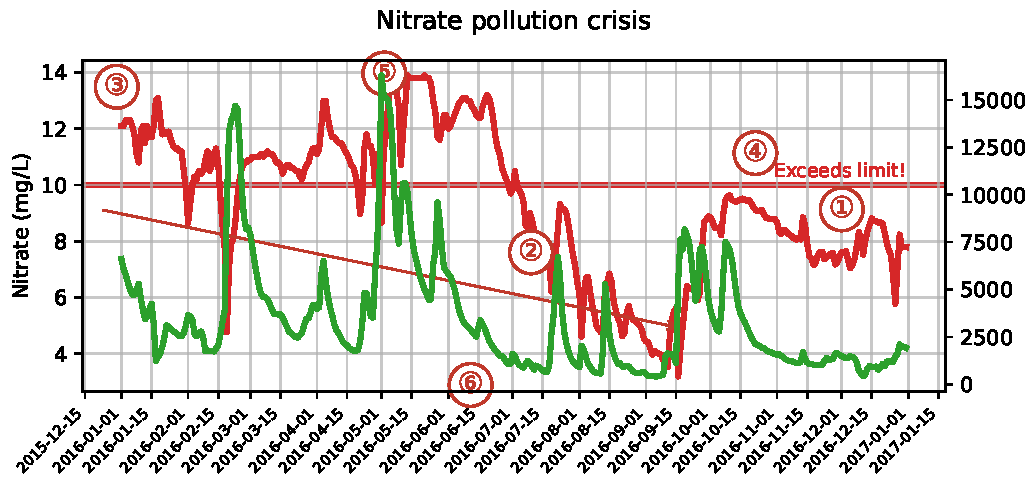
\includegraphics[width=\linewidth]{figures/ch01/ch01-03-nitrate-draft-vague-en.pdf}
\caption{Typical data-plot defects under a vague request (constructed from the real USGS daily record as a counterexample). Here (1) twin axes with red--green coloring, (2) straight lines bridging missing days, (3) incomplete units, (4) a drinking-water reference line labeled ``Exceeds limit!'', (5) a conclusion-laden title, and (6) crowded date ticks all invite misreading.}\label{fig:ch01-03}
\end{figure}

Checking Figure~\ref{fig:ch01-03} against the brief reveals six clear defects marked by red circles: (1) Red--green twin Y axes with unconverted $\text{ft}^3/\text{s}$ discharge create arbitrary curve intersections that falsely suggest concentration and flow are ``equal,'' while clashing for color-vision-deficient readers; (2) the missing days on September 18--19 and December 14 (indicated by thin arrows) are bridged by straight lines, fabricating three days of observations; (3) the left axis omits ``as N'' and the right axis lacks units or any distinction for winter ice estimates; (4) $y=10$ is drawn as a bold red line labeled ``Exceeds limit!'', misapplying a drinking-water standard to untreated river water; (5) the title ``Nitrate pollution crisis'' imposes a conclusion on the reader; and (6) biweekly full-date labels crowd the horizontal axis over a heavy grid.

Now consider the brief-driven workflow. After uploading \path{raccoon-2016-daily.csv} to \scidraw{} scientific visualization (\sdtool{sci-vis}), Lin submits a structured instruction:

\begin{Prompt}
Read the uploaded raccoon-2016-daily.csv. date is calendar date; nitrate_mgL_as_N is
daily mean nitrate plus nitrite (mg/L as N); discharge_cfs is daily mean flow (ft3/s).
Plot two vertically stacked subplots sharing the horizontal time axis (no twin Y axes):
Top subplot: line plot of daily nitrate; y-axis "Nitrate (mg/L as N)"; draw a dashed
gray horizontal line at 10 labeled "US EPA drinking-water MCL (reference only)".
Bottom subplot: convert discharge to m3/s (multiply by 0.028316846592) on a log scale;
y-axis "Discharge (m3/s, log scale)"; highlight dates where discharge_qual is A:e
with a lighter wide band and legend "Light: ice-affected estimates".
Leave missing nitrate dates as visible line breaks; do not interpolate, smooth, or drop rows.
Format x-axis with monthly ticks Jan-Dec 2016. Use one colorblind-safe color per panel.
Omit figure titles and evaluative labels such as "exceeds limit" or "crisis".
\end{Prompt}

Executing deterministic plotting under these rules yields the revised data panel (Figure~\ref{fig:ch01-04}).

\begin{figure}[htbp]\centering
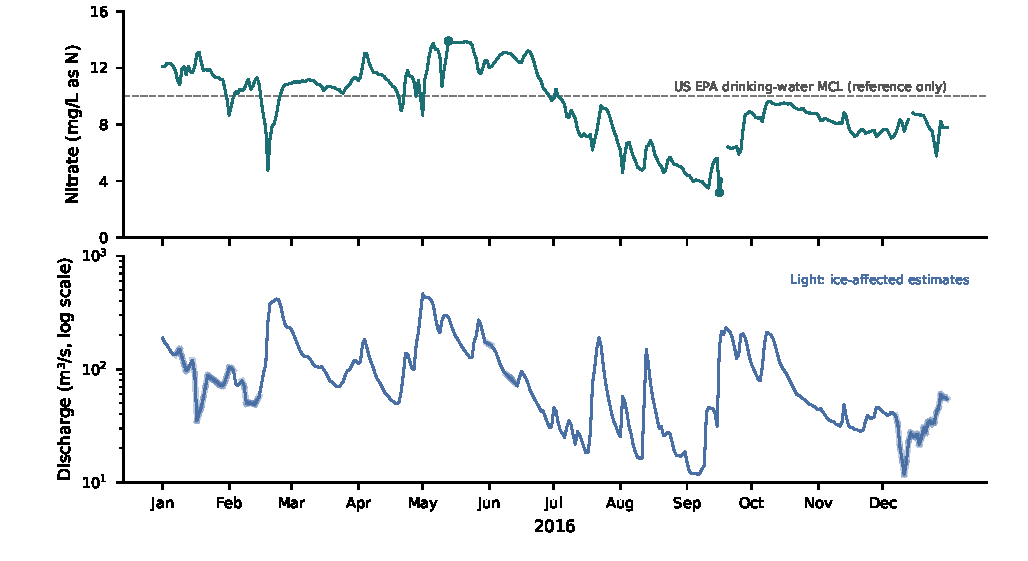
\includegraphics[width=\linewidth]{figures/ch01/ch01-04-nitrate-panel-brief-en.pdf}
\caption{The same dataset replotted from the brief. Top: daily mean nitrate plus nitrite ($\text{mg/L as N}$), with line breaks at the missing days (September 18--19 and December 14); the dashed grey line marks the US EPA drinking-water Maximum Contaminant Level of $10\ \text{mg/L as N}$, shown for reference only because it does not apply to untreated river water. Bottom: daily mean discharge converted from $\text{ft}^3/\text{s}$ to $\text{m}^3/\text{s}$ on a logarithmic scale; lighter segments indicate winter ice-affected estimates. Data: USGS station 05484500, Raccoon River at Van Meter, Iowa, approved daily values downloaded October 29, 2026.}\label{fig:ch01-04}
\end{figure}

Comparing Figure~\ref{fig:ch01-04} with Figure~\ref{fig:ch01-03}, all six defects are resolved: stacked subplots sharing a monthly axis eliminate false curve crossings and allow direct vertical comparison of flow pulses and nitrate responses; the top curve breaks cleanly at the three missing dates and marks the annual maximum ($13.9\ \text{mg/L}$ on May 13) and minimum ($3.19\ \text{mg/L}$ on September 16); the $10\ \text{mg/L}$ line is a muted gray dashed reference; and the bottom panel uses a logarithmic $\text{m}^3/\text{s}$ scale with a lighter band marking the 58 ice-affected days. The unsmoothed plot also preserves an important empirical fact: although monthly mean nitrate was highest in May ($12.84\ \text{mg/L}$) and lowest in September ($5.36\ \text{mg/L}$), January concentrations were also high ($11.75\ \text{mg/L}$). Avoiding smoothing and biased titles lets the true seasonal record stand on its own.

\textbf{Stage 3 (continued): Make a draft---contrasting vague and brief-driven study-area schematics.} Next, we build panel a, the study-area schematic. First consider what happens when an image generator receives only a broad one-line prompt:

\begin{Prompt}
Illustration of nitrate pollution in an agricultural river watershed. Aspect ratio 4:3.
\end{Prompt}

Many people assume that vague prompts mainly risk garbled pseudo-text or smoking factory chimneys. When we generated three images from this exact prompt, the results taught a more important lesson: none of the three runs produced factory smokestacks or dead fish, and the English labels and arrows were largely readable; yet to illustrate ``pollution,'' the model invented \textbf{facilities and ecological mechanisms unsupported by our case materials}. Figure~\ref{fig:ch01-05} shows a representative output, with red circles 1--4 marking four specific problems.

\begin{figure}[htbp]\centering
\begin{tikzpicture}
\node[anchor=south west,inner sep=0] (img) at (0,0) {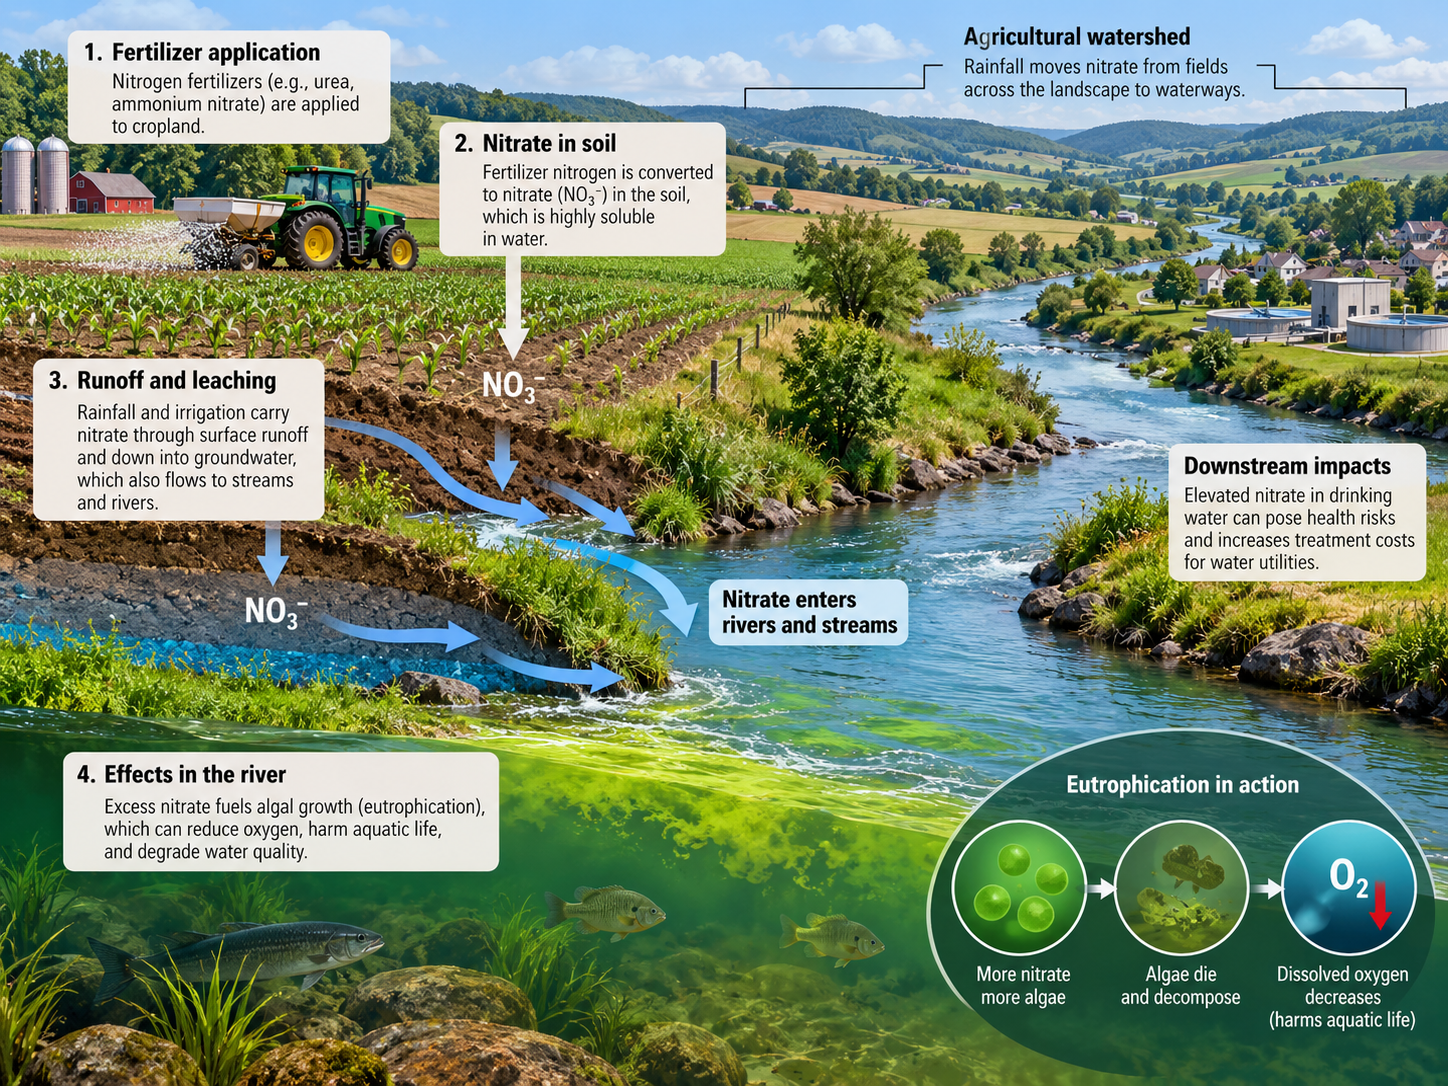
\includegraphics[width=\linewidth]{figures/ch01/ch01-05-site-schematic-vague.png}};
\begin{scope}[x={(img.south east)},y={(img.north west)}]
  \tikzset{badmark/.style={draw=red!80!black,very thick,circle,fill=white,fill opacity=0.88,text opacity=1,text=red!80!black,font=\bfseries\small,inner sep=1.2pt}}
  \node[badmark] at (0.88,0.72) {1};
  \node[badmark] at (0.80,0.22) {2};
  \node[badmark] at (0.22,0.80) {3};
  \node[badmark] at (0.62,0.45) {4};
\end{scope}
\end{tikzpicture}
\caption{A study-area schematic generated from a one-line prompt (the example images in this chapter were generated by an image model; prompts and generation logs are available in the book repository). Without generating factory chimneys or gibberish text, the model still added content unsupported by our case materials: (1) a water-treatment complex with circular tanks, town buildings, and utility-cost claims on the right bank; (2) foreground algal blooms, underwater fish, and a lower-right ``eutrophication---algal decomposition---dissolved oxygen depletion'' diagram (while omitting subsurface tile drains from the left soil cut-away); (3) photorealistic landscape and underwater views with large English text boxes baked into the bitmap; and (4) runoff arrows without the downstream USGS monitoring station or sensor.}\label{fig:ch01-05}
\end{figure}

Examining these four defects one by one shows why the image fails scientific review:
\begin{itemize}
\item \textbf{Problem (1) (Unsupported water-treatment plant and cost claims):} On the right bank (circle 1), the model drew a town and a water-treatment facility with two circular basins, alongside text discussing drinking-water risks and utility treatment costs. Our dataset contains no water-plant locations or cost records; including them misleads readers about the scope of the paper.
\item \textbf{Problem (2) (Unmeasured eutrophication mechanism and omitted tile drains):} The foreground and lower-right inset (circle 2) depict dense green algal blooms, fish, and a causal diagram ($\text{nitrate increase} \rightarrow \text{algal decomposition} \rightarrow \text{dissolved oxygen } [\text{O}_2] \text{ drop}$), whereas the soil cut-away on the left shows only surface runoff and groundwater, omitting the subsurface tile drains central to this watershed. Presenting unmeasured downstream ecological effects as fact while leaving out the primary transport pathway is a serious scientific distortion.
\item \textbf{Problem (3) (Photorealistic decoration and text locked in bitmap pixels):} The scene (circle 3) uses realistic skies, a distant tractor, and underwater lighting, with four large English text blocks rasterized directly into the bitmap where their font size, style, and wording cannot be edited separately.
\item \textbf{Problem (4) (Missing monitoring station location):} Although runoff arrows are present, the downstream channel (circle 4) lacks the USGS 05484500 monitoring station and in-situ sensor needed to link panel a to the data in panel b.
\end{itemize}

Keeping a schematic faithful to the science requires two rules: first, specify \textbf{required scientific objects} alongside a \textbf{strict exclusion list}; second, require a \textbf{clean base image with zero embedded text}, adding vector labels later in a layout or typesetting tool. Below is the core portion of the structured prompt (the full prompt is in the \texttt{cases/} directory of the book repository):

\begin{Prompt}
Flat 2D scientific schematic for a journal figure panel, portrait 4:5, pure white
background. Clean vector style: flat fills, thin dark-gray outlines, no gradients,
no shadows, no 3D, no texture.
ABSOLUTELY NO TEXT: no letters, words, numbers, symbols, labels, legend, or title.
SCENE: simplified oblique (~30-degree) view of an agricultural landscape with a
cut-away soil block in the lower-left quarter.
- Upper half: 5-6 rectangular fields in muted sage green and wheat yellow; no buildings.
- Meandering river (soft blue) from upper-left to lower-right, joined by one tributary ditch.
- Lower-left soil cut-away: 3 round gray subsurface drain pipes, one outlet discharging
  into the tributary ditch.
- Lower-right river bank: simple gray monitoring station box with cable to a submerged
  cylindrical sensor; 2-3 hollow chevrons on water surface pointing downstream.
STRICTLY EXCLUDE: factories, chimneys, sewage pipes, towns, bridges, dead fish, algae,
murky water, warning signs, chemical symbols, clouds, decorative borders.
\end{Prompt}

Even with a detailed prompt, every candidate output must be inspected against the brief. We generated three images from this prompt and found distinct differences: in the first run, a white gap broke the connection between the receiving channel beside the soil cut-away and the tributary ditch joining the main river, severing the ``tile drain $\rightarrow$ ditch $\rightarrow$ river'' pathway, so it was rejected; in the third run, two separate tributary ditches entered the main channel independently, departing from our single-ditch design, so it too was rejected; only the second run delivered a white background, zero text, six cropland fields, three gray drain-pipe cross-sections, a continuous tributary ditch entering the main river, the downstream monitoring box and sensor, and three white downstream V-chevrons, with no excluded objects.

Zooming in to 200\% on that second image still reveals four minor deviations: the ditch forms a small Y-junction before entering the river; the third drain pipe on the right doubles directly as the flowing outlet; the sensor rests at the water surface with ripples rather than appearing deeply submerged; and the soil block and station box retain subtle grain texture and shading. Because none of these details alter the core topological pathway---cropland to subsurface tile drains to ditch to main channel to gauge---and the image is free of pseudo-text, we can note ``Schematic, not to scale'' in the legend and overlay six vector labels in LaTeX to obtain a sound study-area panel (Figure~\ref{fig:ch01-06}).

\begin{figure}[htbp]\centering
\begin{tikzpicture}
\node[anchor=south west,inner sep=0] (img) at (0,0) {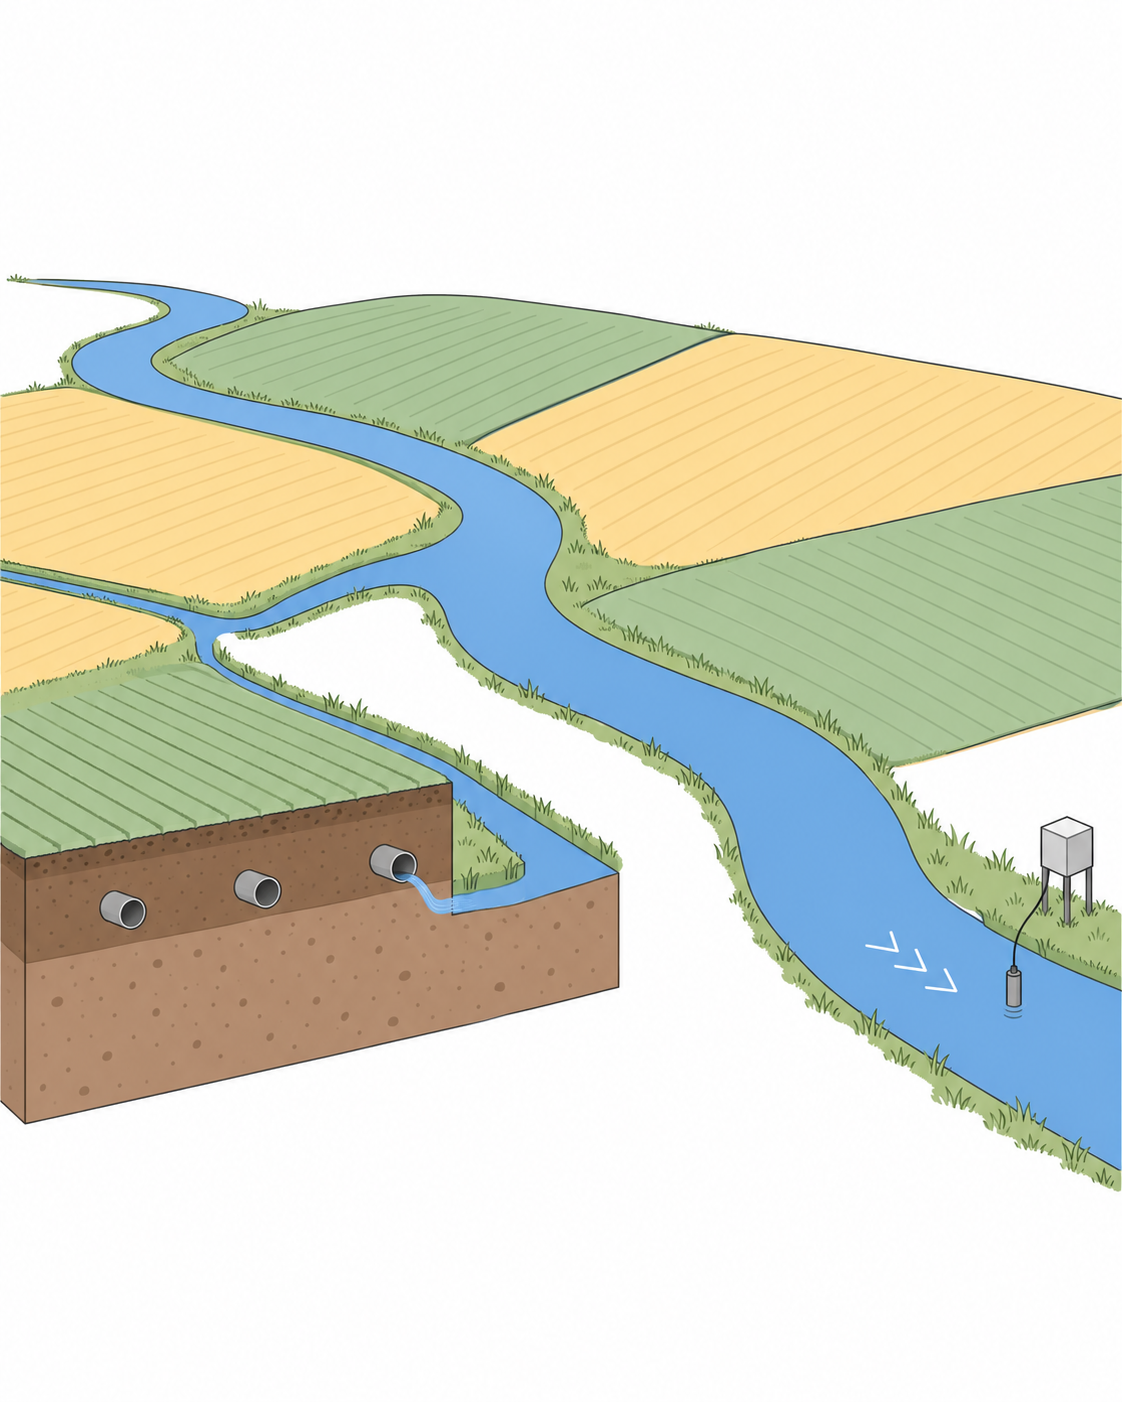
\includegraphics[width=0.62\linewidth]{figures/ch01/ch01-06-site-schematic-brief.png}};
\begin{scope}[x={(img.south east)},y={(img.north west)}]
  \tikzset{lbl/.style={font=\footnotesize,fill=white,fill opacity=0.82,text opacity=1,inner sep=1.5pt,align=center}}
  \node[lbl] at (0.50,0.88) {Cropland (corn--soybean, schematic)};
  \node[lbl] at (0.22,0.18) {Subsurface tile drains};
  \node[lbl] at (0.12,0.45) {Drainage ditch};
  \node[lbl] at (0.55,0.55) {Raccoon River};
  \node[lbl] at (0.80,0.12) {USGS 05484500 station};
  \node[lbl] at (0.72,0.36) {Flow};
\end{scope}
\end{tikzpicture}
\caption{The study-area schematic base generated from the brief (the second of three runs) with English labels overlaid afterward. The base image contains no generated text, excludes unrelated facilities and unverified ecological effects, and clearly shows the spatial pathway from cropland and subsurface tile drains through the drainage ditch into the Raccoon River and down to the monitoring station.}\label{fig:ch01-06}
\end{figure}

\textbf{Stage 4: Check and revise---managing iterations with a revision list.} Instead of asking a tool to ``make it look more professional,'' compare the data draft (Figure~\ref{fig:ch01-03}) and schematic draft (Figure~\ref{fig:ch01-05}) against the brief and log every problem in a structured \textbf{revision list} specifying the verifiable fix and the stage to return to:

\begin{center}\footnotesize
\setlength{\tabcolsep}{3pt}
\renewcommand{\arraystretch}{1.15}
\begin{tabularx}{\linewidth}{@{}c>{\raggedright\arraybackslash}p{32mm}>{\raggedright\arraybackslash}p{22mm}Y>{\raggedright\arraybackslash}p{22mm}@{}}
\toprule
\textbf{\#} & \textbf{Defect found in draft} & \textbf{Clause violated} & \textbf{Verifiable revision instruction} & \textbf{Stage to return to} \\
\midrule
1 & Twin Y axes make curve crossings look like ``equal concentration and flow'' & [Objects and relationships] & Split into two vertically stacked subplots sharing the horizontal time axis & Make a draft \\
2 & Missing days (Sep 18--19, Dec 14) bridged by straight lines & [Limits], [Acceptance] & Keep empty cells as \texttt{NaN} so the curve breaks naturally at all three gaps without interpolation & Gather materials (check parser logic) \\
3 & Axis label omits ``as N''; discharge lacks units and conversion & [Materials], [Limits] & Write full units; multiply discharge by $0.028316846592$ to $\text{m}^3/\text{s}$ on a log axis & Gather materials \\
4 & $10\ \text{mg/L}$ line labeled ``Exceeds limit!''; conclusion-laden title at top & [Limits] & Remove title; change to dashed gray line labeled ``drinking-water MCL (reference only)'' & Define the task (clarify scope) \\
5 & High-saturation red--green palette; crowded biweekly date strings & [Visual style] & Use one colorblind-safe hue per subplot; use monthly ticks Jan--Dec & Make a draft \\
6 & Winter 58 days of ice-affected estimated flow (\texttt{A:e}) indistinguishable from measured flow & [Goal] & Highlight \texttt{A:e} dates with a lighter wide line and add a subplot legend & Make a draft \\
7 & Schematic draft adds water plant, algal bloom, and eutrophication inset while omitting tile drains & [Objects and relationships], [Limits] & Do not patch locally; regenerate a text-free base from the brief's object and exclusion lists & Make a draft \\
8 & Schematic text baked into bitmap, with broken ditch in run 1 and two ditches in run 3 & [Visual style], [Objects and relationships] & Forbid text in base image; select run 2 with continuous ditch path and overlay vector labels & Check and revise \\
\bottomrule
\end{tabularx}
\end{center}

Keep one iron rule in mind: \textbf{after every revision, re-verify the entire figure from scratch, including parts you did not ask to change.} Generative redrawing can fix a drainage ditch while dropping the monitoring station, and adjusting axis padding in a script can clip the annual peak. Three habits keep re-verification reliable: first, place the old and new versions side by side (or flip rapidly between them) to spot unintended drift in unchanged areas; second, check the extreme dates and gap dates from the data dictionary directly on the plot to confirm that peaks, troughs, and breaks sit at the exact dates; third, zoom to 200\% to recount key scientific objects and connection directions against the acceptance checklist.

\textbf{Stages 5 and 6: Assemble and explain, final-size inspection, and delivery.} Once both panels pass verification, move to Stage 5, ``Assemble and explain.'' In \scidraw{}, download the schematic and data panels to your local folder, open the multi-panel assembly tool (\sdtool{multi-panel-figure-maker}), select a $1 \times 2$ grid with an approximate $36:62$ width ratio between left panel \textbf{a} and right panel \textbf{b}, apply automatic bold lettering \textbf{a}/\textbf{b} and the $174\ \text{mm}$ double-column journal width preset, and export a ZIP package containing TIFF, PNG, PDF, PPTX, and processing records. Aligning the two panels produces the complete Figure 2 (Figure~\ref{fig:ch01-07}).

\begin{figure}[htbp]\centering
{\makeatletter\tikzset{text width/.code={\def\tikz@text@width{#1\textwidth}}}\makeatother\begin{tikzpicture}
\node[anchor=south west,inner sep=0] (panel) at (0,0) {%
  \begin{minipage}[t]{0.34\linewidth}
    \IfFileExists{figures/ch01/ch01-06-site-schematic-brief.png}{%
      \begin{tikzpicture}
      \node[anchor=south west,inner sep=0] (img) at (0,0) {%
        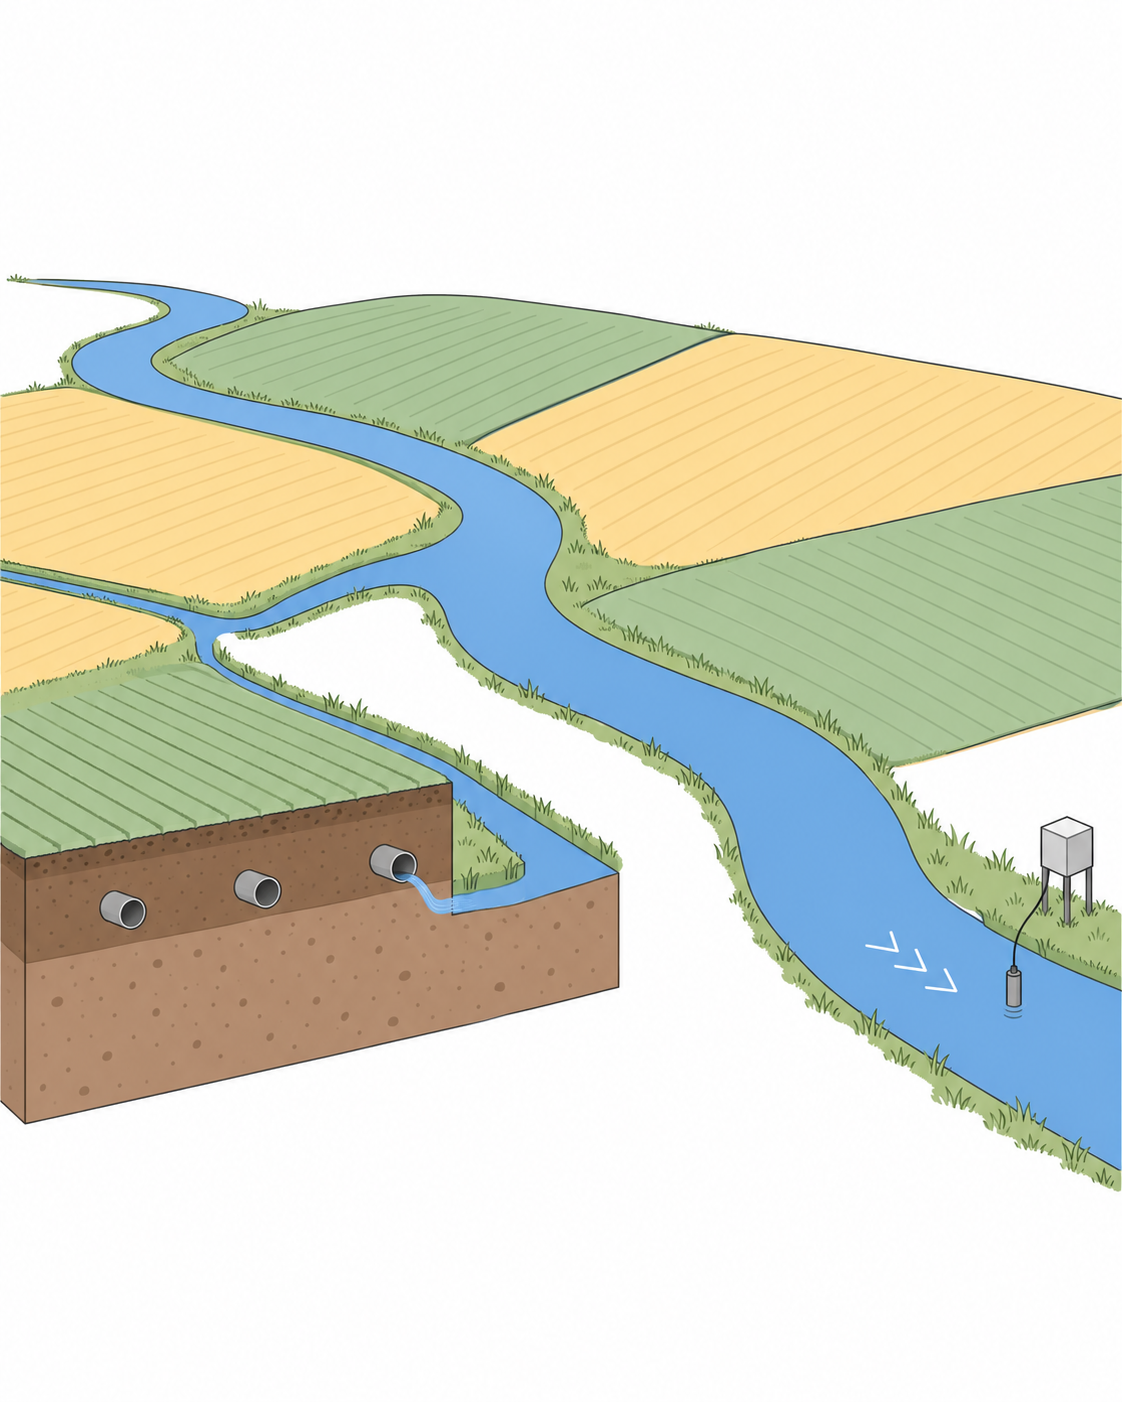
\includegraphics[width=\linewidth]{figures/ch01/ch01-06-site-schematic-brief.png}};
      \begin{scope}[x={(img.south east)},y={(img.north west)}]
        \tikzset{lbl/.style={font=\scriptsize,fill=white,fill opacity=0.8,text opacity=1,inner sep=1pt,align=center}}
        \node[lbl,text width=0.28,align=center] at (0.48,0.86) {Cropland (corn--soybean, schematic)};
        \node[lbl,text width=0.22,align=center] at (0.20,0.16) {Subsurface tile drains};
        \node[lbl,text width=0.18,align=center] at (0.10,0.44) {Drainage ditch};
        \node[lbl,text width=0.22,align=center] at (0.52,0.52) {Raccoon River};
        \node[lbl,text width=0.26,align=center] at (0.52,0.10) {USGS 05484500 station};
        \node[lbl] at (0.50,0.38) {Flow};
      \end{scope}
      \end{tikzpicture}
    }{%
      \fbox{\parbox[c][0.36\linewidth][c]{0.34\linewidth}{\centering\scriptsize Missing ch01-06 base\\(codex-image; out of scope)}}
    }
    \par\vspace{1mm}{\scriptsize Schematic, not to scale}
  \end{minipage}\hfill
  \begin{minipage}[t]{0.64\linewidth}
    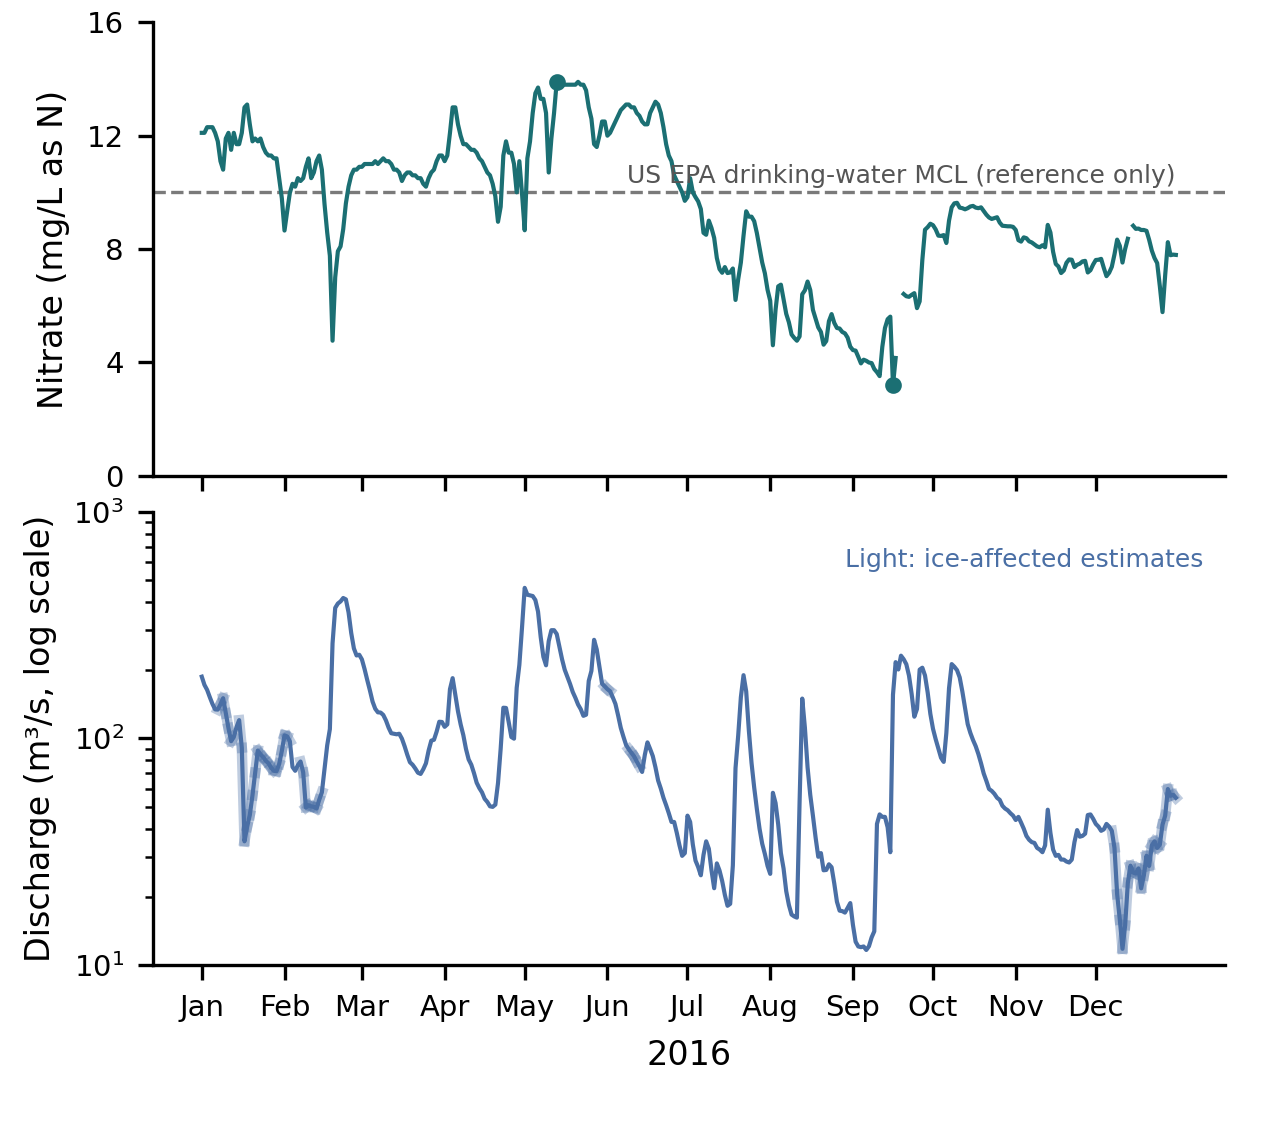
\includegraphics[width=\linewidth]{figures/ch01/ch01-04-nitrate-panel-brief-en-panel.png}
  \end{minipage}};
\node[anchor=south west,font=\bfseries\small] at ([xshift=1mm,yshift=1mm]panel.north west) {a};
\node[anchor=south west,font=\bfseries\small] at ([xshift=0.34\linewidth,yshift=1mm]panel.north west) {b};
\end{tikzpicture}
}
\caption{\textbf{Example Figure 2: nitrate concentration and discharge in the Raccoon River, 2016.} (a) Simplified study-area schematic: subsurface tile drainage from cropland enters the river channel via a ditch, with the USGS monitoring station (05484500, Van Meter, IA) downstream; not to scale, and does not represent specific fields, pipe networks, or pollution sources. (b) Top: daily mean nitrate plus nitrite ($\text{mg/L as N}$), with breaks at missing days; the dashed grey line marks the US EPA drinking-water Maximum Contaminant Level of $10\ \text{mg/L}$ (as N), for reference only. Bottom: daily mean discharge ($\text{m}^3/\text{s}$, converted from $\text{ft}^3/\text{s}$, logarithmic scale), with lighter segments indicating winter ice-affected estimates. Data are USGS approved daily values (public domain), downloaded October 29, 2026; no load calculation or statistical test is included. The schematic base was generated by an image model and labels were overlaid by the author; prompts and generation logs for this chapter's example figures are available in the book repository.}\label{fig:ch01-07}
\end{figure}

Next, write the figure legend. When uploading the final figure to the legend assistant (\sdtool{figure-legend}) to draft an outline, remember that \textbf{the model sees only image pixels and cannot know station numbers, download dates, conversion formulas, or regulatory boundaries.} The author must personally verify and add four things: (1) station ID 05484500, location, approved status, and download date; (2) ``as N'' units, gap breaks, $\text{m}^3/\text{s}$ log scaling, and the meaning of ice-affected segments; (3) statements that panel a is ``not to scale, and does not represent specific fields, pipe networks, or pollution sources,'' that the $10\ \text{mg/L}$ line is ``for reference only,'' and that ``no load calculation or statistical test is included'' (never fabricating sample sizes or test statistics); and (4) disclosure that the schematic base was made with a generative tool and labeled by the author.

Finally, in Stage 6 (``Check and deliver''), inspect the figure at 100\% of its $174\ \text{mm}$ print width to confirm that all text is $\ge 6\ \text{pt}$ and no overlaid labels obscure the drain pipes or monitoring station. Then run the technical checker (\sdtool{figure-checker}) to test resolution, color space, grayscale contrast, and color-vision accessibility. Remember that \textbf{passing a technical check does not mean the science is correct}; always verify every data point, break, and legend claim against the `[Acceptance]` criteria before archiving.

\section{Choosing a route in SciDraw AI}

The figure workflow guide (\sdtool{figure-workflow}) in \scidraw{} first asks which kind of figure you are making: \textbf{Mechanism \& workflow diagram, Data figure, Multi-panel figure, or Graphical abstract} (Figure~\ref{fig:ch01-08}). Once you pick one, the page shows a short ordered route of three or four steps, each with a one-sentence description and a button that opens the matching tool. The mechanism route, for example, runs: Generate a first draft (mechanism diagram generator, or the flow diagram generator for a flowchart) $\rightarrow$ Refine details (AI Drawing) $\rightarrow$ Write the figure legend (legend tool) $\rightarrow$ Check and export (figure checker). Each step works on its own, so if you already have a draft you can start at step 2.

\begin{figure}[htbp]\centering
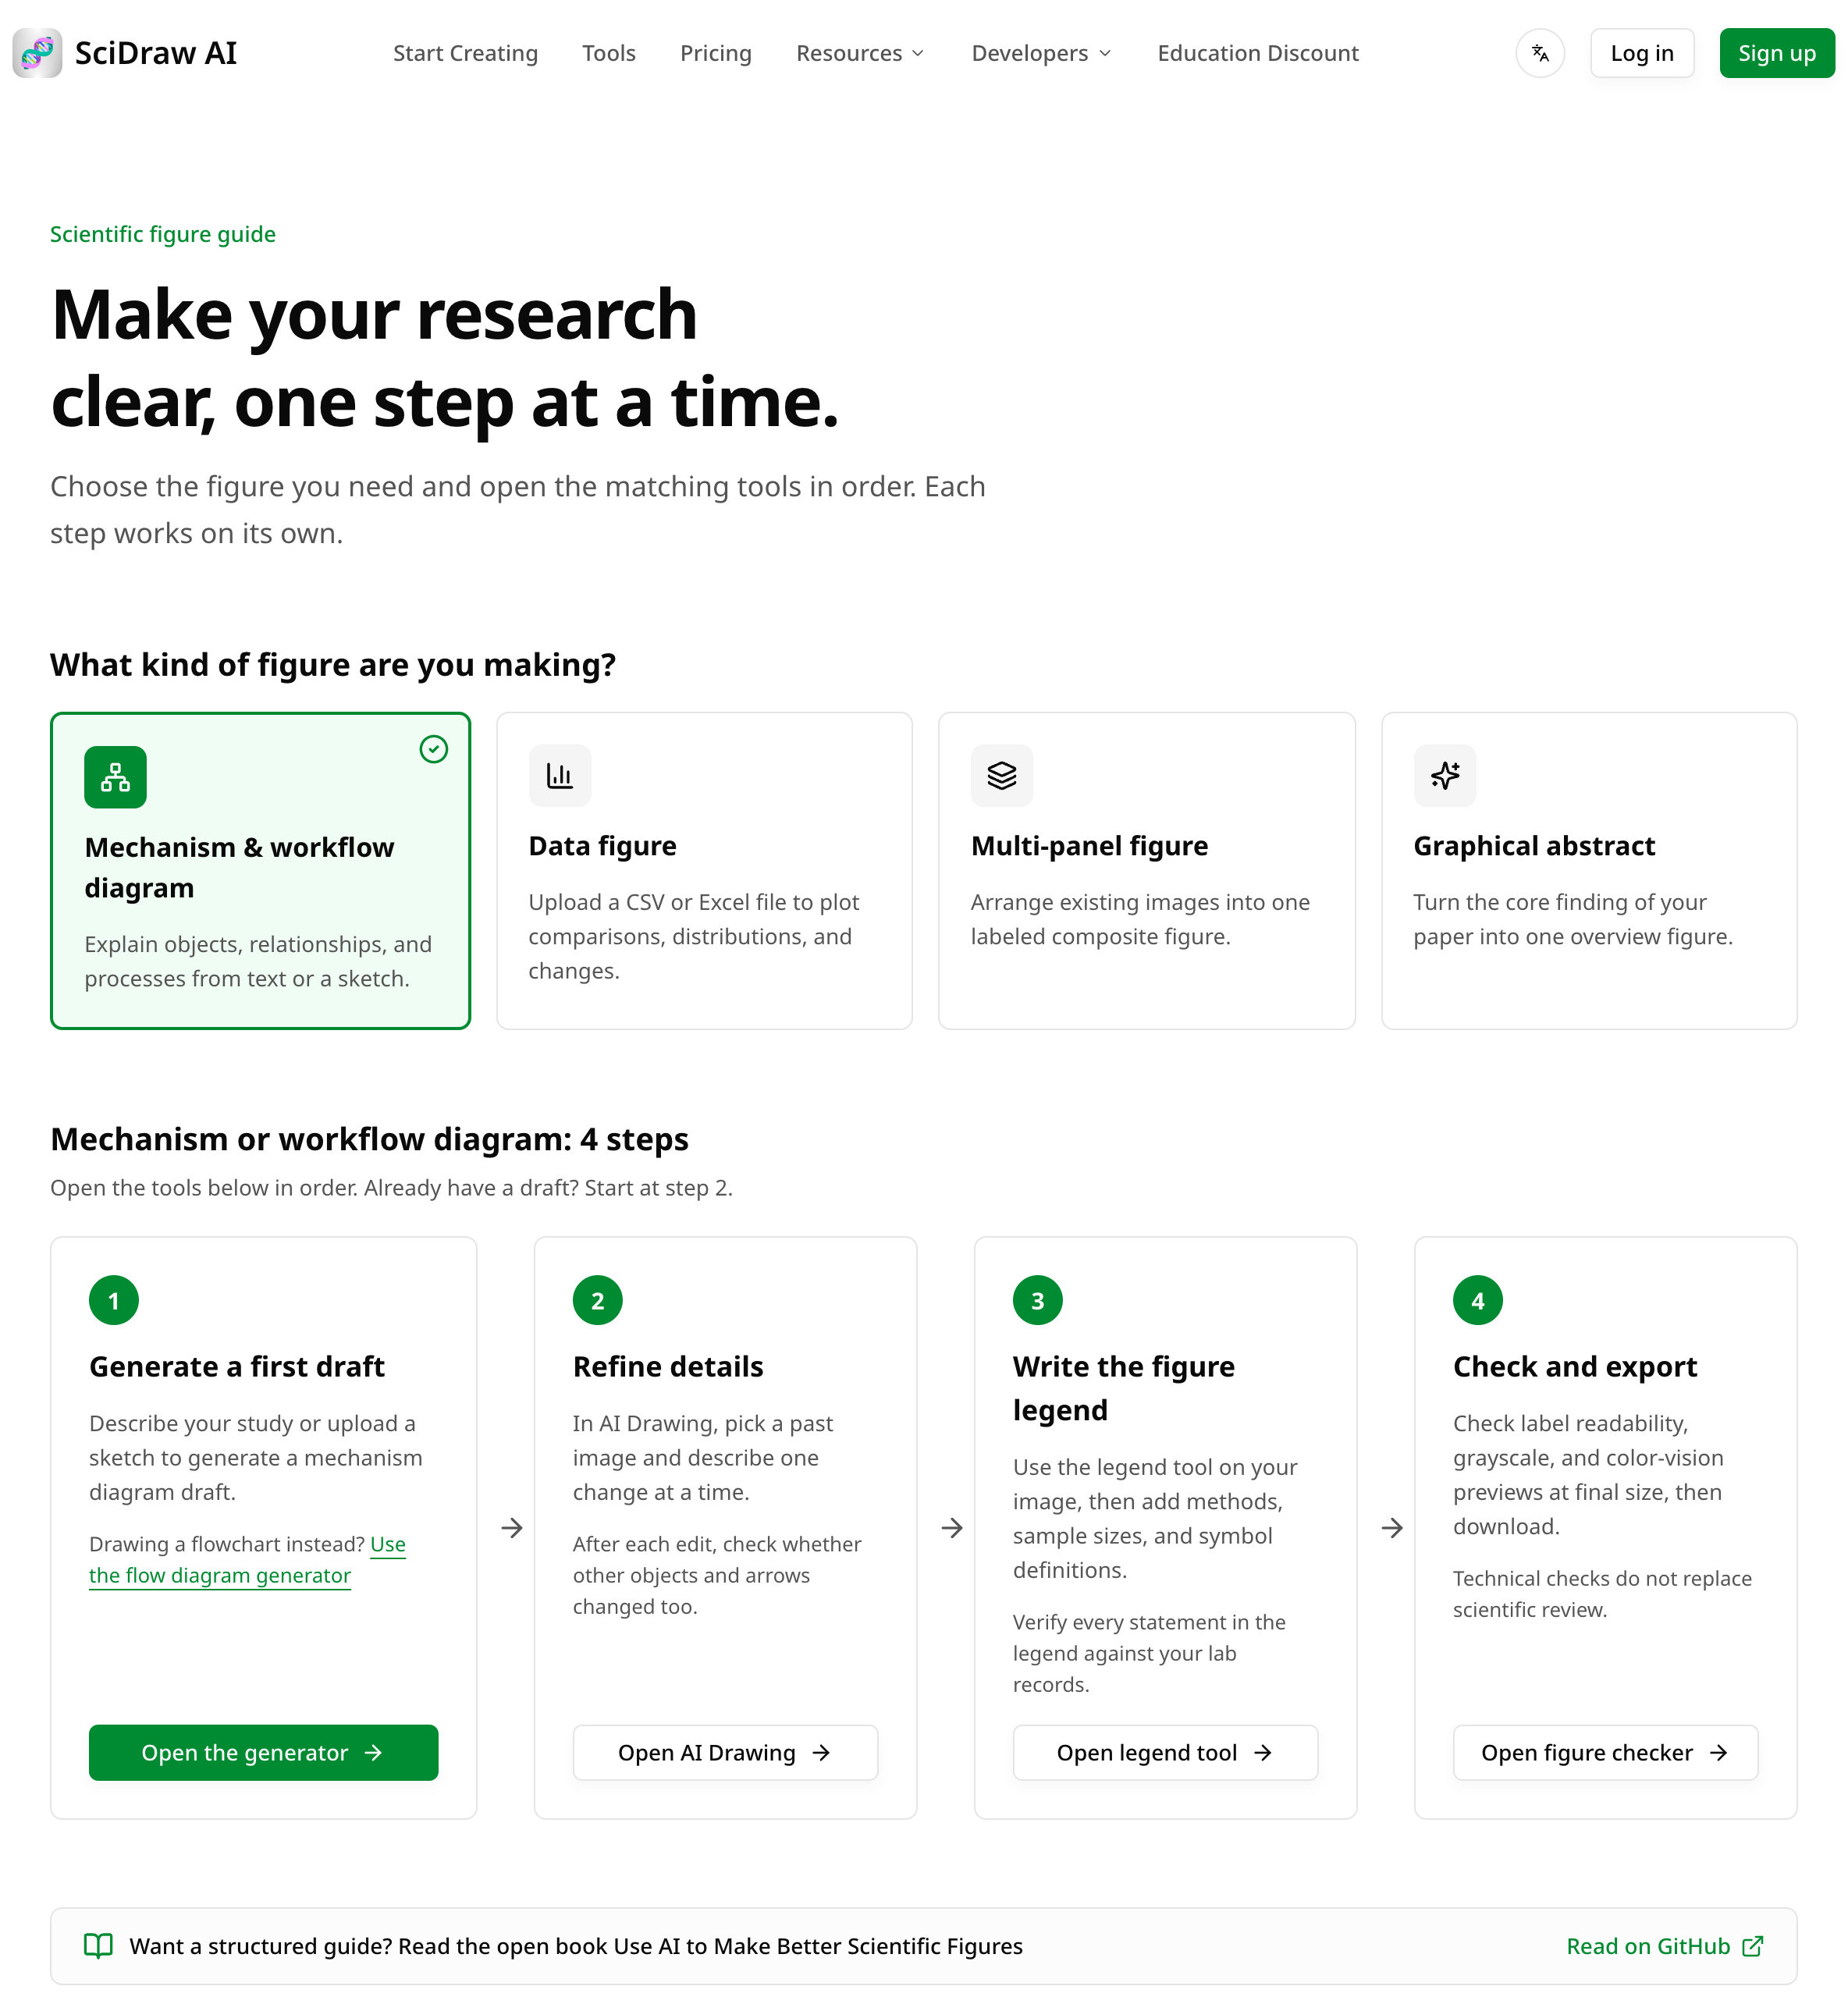
\includegraphics[width=0.92\linewidth,height=0.68\textheight,keepaspectratio]{figures/ch01/ch01-08-guide-ui-en.png}
\caption{The \scidraw{} figure workflow guide (30 October 2026). With ``Mechanism \& workflow diagram'' selected, the page lists a four-step route---Generate a first draft, Refine details, Write the figure legend, Check and export---each with one sentence and a button that opens the tool.}\label{fig:ch01-08}
\end{figure}

A composite figure can chain two routes together: our case followed the ``Data figure'' route into \sdtool{sci-vis} for panel b, then the ``Mechanism \& workflow diagram'' route into \sdtool{workflow-diagram-generator} or \sdtool{ai-drawing} for panel a, before moving to the panel assembly, legend, and checking tools. If you already have a finished plot and only need a legend or resolution check, you can jump directly to that step.

Keep three platform facts in mind when using the guide:
\begin{enumerate}
\item \textbf{The guide stores neither your brief nor your progress:} The page only shows the route and links to the tools; it has no brief editor and does not track which step you have reached. Write the brief in your own document or text file, keep it in the project folder as the record, and paste it into the tool at each step.
\item \textbf{Cross-tool handoff uses download and upload:} The guide's buttons simply open the matching tool; they do not carry your brief or images along. When sending individual panels to the assembly, legend, or checking tools, download clearly named files (such as \texttt{panel-b-nitrate-v2.pdf}) and upload them to the next tool, which also avoids passing outdated drafts.
\item \textbf{The guide does not perform scientific review for you:} It supplies only the order of steps and the tool links; verifying units, quality codes, and evidential boundaries remains the author's job.
\end{enumerate}

\section{Keep a small archive for every figure}

Creating a small folder with a fixed structure on your local drive or code repository for each figure makes it easy to reproduce or revise months later when reviewers ask for changes. The archive structure for this chapter's case is:

\begin{Prompt}
fig2-raccoon-nitrate/
  source/   usgs-05484500-2016.rdb (raw download backup, read-only)
            raccoon-2016-daily.csv, data-dictionary.md (fields, units, flags, DOI, date)
  brief/    figure2-brief-v1.txt (your saved brief), prompts-log.txt (all submitted inputs)
  drafts/   panel-b-draft1.pdf, panel-b-revised.pdf, panel-a-candidates/,
            revision-notes.md (the 8 draft defects and return-path revision log)
  final/    figure2-final.pdf, figure2-final.tiff, legend-zh.txt, legend-en.txt,
            ai-use.md (functions used, dates, inputs, adopted outputs, manual edits), checks.md
  code/     fetch_usgs.py, plot_nitrate.py
\end{Prompt}

You do not need to log every mouse movement, but \textbf{every decision that affects scientific facts or quantitative interpretation must leave a record}: unit conversion formulas and axis transformations, rules for missing values and quality codes, reasons for removing unsupported elements and selecting among generated candidates, and the scope of reference lines. In \texttt{ai-use.md}, record the tool functions used, date, actual inputs, adopted outputs, and manual edits; check your target journal's current AI disclosure policy before submission.

\section{What AI can and cannot do at this stage}

The boundaries among AI, deterministic tools, and the author across the six stages are summarized in Table~\ref{tab:ch01-01}.

\begin{table}[htbp]\centering\footnotesize
\setlength{\tabcolsep}{3pt}
\renewcommand{\arraystretch}{1.15}
\caption{What AI can do, what AI cannot do, and what the author must check across the six stages.}\label{tab:ch01-01}
\begin{tabularx}{\linewidth}{@{}>{\raggedright\arraybackslash}p{20mm}YYY@{}}
\toprule
\textbf{Stage} & \textbf{What AI can do} & \textbf{What AI cannot do} & \textbf{What the author must check} \\
\midrule
Define the task & Draft brief fields from your description; point out missing items (such as units, audience, or size) & Decide the research question the figure should answer; judge whether a claim holds & Whether the task sentence is testable; whether intended use and dimensions are accurate \\
Gather materials & Write download/parsing scripts; tally missing values and quality codes; draft data dictionary & Guarantee the dataset version is right; tell ``as N'' from ``as $\text{NO}_3^-$'' without reading parameter docs & Units, quality codes, download date, and whether provisional data were mixed in \\
Make a draft & Data plots: plot from explicit instructions; schematics: quickly generate layout candidates & Guarantee no interpolation or smoothing unless told; guarantee schematics omit unsupported objects & Check against acceptance criteria line by line; count raw points; look for added objects \\
Check and revise & Execute specific revision commands; regenerate plots or images from a defect list & Judge whether an edit introduced new errors; change one spot without affecting the rest of an image & Re-verify the entire figure after every edit, including parts not meant to change \\
Assemble and explain & Grid layout, panel lettering, size presets; draft figure legends & Know station IDs, download dates, or processing rules invisible in the image; fabricating sample sizes or statistics is forbidden & Whether every number and statement in the legend has a documented source \\
Check and deliver & Technical checks (resolution, color mode, grayscale, color-vision risks) & Scientific peer review; confirm journal AI policies for you & Readability at final print size; whether others can reproduce the figure from the delivery pack \\
\bottomrule
\end{tabularx}
\end{table}

\section{Checklist}

\begin{itemize}
\item I can write the goal of this figure in one sentence, and it constrains the chart type, layout, or labels.
\item I have identified the material category of each panel; data panels use deterministic plotting, and schematic panels depict no unsupported objects.
\item An unaltered copy of the raw data is preserved; units, quality codes, missing values, and download dates are written in the data notes.
\item Every input actually submitted to a tool has been saved.
\item Every revision round is recorded: what changed, why, and which stage the workflow returned to.
\item The final figure has been checked for text and line legibility at its actual print dimensions.
\item Every number, source, and processing note in the figure legend is backed by the archive.
\item I moved on from each step only after checking its output against the brief, not merely because a tool page had been opened.
\item The delivery package includes an AI-use log, and I checked the target journal's current requirements before submission.
\end{itemize}

\section{Exercises}

\begin{enumerate}
\item \textbf{(Task sentences)} Write two alternative task sentences for this chapter's case: one focused on ``how many days high concentrations persist in spring,'' and another focused on ``concentrations during low-flow periods.'' Explain how each would change the chart type, time range, or annotations.
\item \textbf{(Finding defects)} Without looking at the revision table in Section 1.4, list at least five problems across Figure~\ref{fig:ch01-03} and Figure~\ref{fig:ch01-05}, write one verifiable revision instruction for each, and state which of the six stages each problem should return to.
\item \textbf{(Hands-on with \scidraw{})} Download one year of daily mean data from another USGS station with a nitrate sensor (or use a time series from your own research). Write a brief in your own document following the format in Section 1.4, then choose ``Data figure'' in the figure workflow guide (\sdtool{figure-workflow}), follow step 1 into \sdtool{sci-vis}, upload the data, and paste in the plotting requirements from your brief. Check the output against your acceptance criteria item by item, record at least one revision instruction and its effect, and archive the entire process using the folder structure in Section 1.6.
\end{enumerate}

\section*{References}

\begin{itemize}
\item Pellerin BA, Stauffer BA, Young DA, Sullivan DJ, Bricker SB, Walbridge MR, Clyde GA, Shaw DM. Emerging tools for continuous nutrient monitoring networks: sensors advancing science and water resources protection. \textit{JAWRA Journal of the American Water Resources Association}. 2016;52(4):993--1008. \url{https://doi.org/10.1111/1752-1688.12386}
\item Rougier NP, Droettboom M, Bourne PE. Ten simple rules for better figures. \textit{PLoS Computational Biology}. 2014;10(9):e1003833. \url{https://doi.org/10.1371/journal.pcbi.1003833}
\item Schilling K, Zhang Y-K. Baseflow contribution to nitrate-nitrogen export from a large, agricultural watershed, USA. \textit{Journal of Hydrology}. 2004;295(1--4):305--316. \url{https://doi.org/10.1016/j.jhydrol.2004.03.010}
\item U.S. Environmental Protection Agency. National Primary Drinking Water Regulations (nitrate MCL 10 mg/L as N). \url{https://www.epa.gov/ground-water-and-drinking-water/national-primary-drinking-water-regulations}
\item U.S. Geological Survey. USGS water data for the Nation: National Water Information System database, site 05484500. \url{https://doi.org/10.5066/F7P55KJN} (accessed 2026-10-29).
\item Weissgerber TL, Milic NM, Winham SJ, Garovic VD. Beyond bar and line graphs: time for a new data presentation paradigm. \textit{PLOS Biology}. 2015;13(4):e1002128. \url{https://doi.org/10.1371/journal.pbio.1002128}
\end{itemize}
